\section{Explicit Examples: Complete Computations of $A_\infty$ Operations}
% label removed: sec:examples_complete

Three fully worked examples follow, with complete computations and explicit integral evaluations.
\subsection{Example I: Free Chiral Multiplet (Complete Treatment)}
% label removed: ex:free_chiral_complete

\subsubsection{Field Content and Classical Action}
A free chiral multiplet on $\R_t \times \C_z$ consists of a complex scalar field $\phi$ (in cohomological degree~$0$) and its BV antifield $\psi$ (in cohomological degree~$1$). The classical action in Euclidean signature is:
\begin{equation}
% label removed: eq:free_action
S_{\text{free}} = \int_{\R \times \C} \left( |\partial_t \phi|^2 + |\dbar \phi|^2 \right) \, dt \wedge dz \wedge d\bar{z}.
\end{equation}
After holomorphic-topological twist, the BV action becomes:
\begin{equation}
S_{\text{HT}} = \int_{\R \times \C} \psi \,(\dbar + d_t)\, \phi \, dt \wedge dz \wedge d\bar{z}.
\end{equation}
\subsubsection{BV-BRST Complex}

In the BV formalism, the field $\phi$ (degree~$0$) is paired with the antifield $\psi$ (degree~$1$) via the BV bracket:
\begin{equation}
\{\phi(x), \psi(y)\}_{\mathrm{BV}} = \delta^{(3)}(x-y).
\end{equation}
The BV-BRST differential $Q = \{S_{\text{HT}}, \cdot\}_{\mathrm{BV}}$ acts on local observables $\A_{\text{free}} = \C[\phi_n, \psi_n \mid n \geq 0]$ by:
\begin{align}
Q \cdot \phi_n &= \psi_n, % label removed: eq:Q_free_phi \\
Q \cdot \psi_n &= 0. % label removed: eq:Q_free_psi
\end{align}
One verifies $Q^2 = 0$ directly: $Q^2\phi_n = Q(\psi_n) = 0$.

Here $\phi_n = \frac{1}{n!} \partial_z^n \phi$ denotes the $n$th holomorphic derivative.
\subsubsection{Propagator and Two-Point Function}
The free propagator in HT gauge is the Green's function for the kinetic operator $d_t + \dbar$:
\begin{equation}
% label removed: eq:free_propagator
\langle \phi(t_1, z_1) \psi(t_2, z_2) \rangle = \frac{1}{2\pi} \cdot \frac{\Theta(t_1 - t_2)}{z_1 - z_2}.
\end{equation}
In the holomorphic direction, this becomes:
\begin{equation}
% label removed: eq:free_propagator_holo
\langle \phi(z_1) \psi(z_2) \rangle_{\text{holo}} = \frac{1}{z_1 - z_2}.
\end{equation}

\subsubsection{Computing $m_2$: The $\lambda$-Bracket}
The binary operation $m_2$ is computed using the two-point function. For observables $O_1 = \phi$ and $O_2 = \psi$:
\begin{equation}
m_2(\phi(z_1), \psi(z_2)) = \oint_{|z_1 - z_2| = \varepsilon} \langle \phi(z_1) \psi(z_2) \rangle \, \frac{dz_1}{z_1 - z_2}.
\end{equation}

Using the propagator \eqref{eq:free_propagator_holo}:
\begin{equation}
m_2(\phi, \psi) = \frac{1}{(z_1 - z_2)},
\end{equation}
so the $\lambda$-bracket is:
\begin{equation}
% label removed: eq:free_lambda_bracket
\{\phi_\lambda \psi\} = 1.
\end{equation}

On cohomology, since $(\phi_n, \psi_n)$ are acyclic doublets with $H^\bullet = \C$, the descended $\lambda$-bracket is trivial:
\begin{equation}
\{\cdot_\lambda \cdot\}_{\text{coh}} = 0.
\end{equation}

\subsubsection{Verification: Higher Operations Vanish}

\begin{proposition}[All $m_{k \geq 3} = 0$ for Free Theory; \ClaimStatusProvedHere]
% label removed: prop:free_higher_vanish
In the free chiral multiplet theory, all higher operations $m_k = 0$ for $k \geq 3$.
\end{proposition}

\begin{proof}
Higher operations $m_k$ arise from Feynman diagrams with $k$ external legs. For $k \geq 3$, such diagrams require at least one internal vertex. However, the free theory has \textbf{no interaction vertices} (the action is quadratic). Therefore, all diagrams contributing to $m_{k \geq 3}$ vanish identically.

Algebraically, this follows from the fact that the free propagator $\langle \phi(z_1)\psi(z_2)\rangle$ satisfies:
\begin{equation}
Q \cdot \text{Prop}(z_1, z_2) = 0 \quad \text{(on-shell)},
\end{equation}
and there are no cubic or higher vertices to generate internal structure.
\end{proof}

\subsubsection{Cohomology and PVA Structure}

\begin{proposition}[Cohomology of Free Theory; \ClaimStatusProvedHere]
% label removed: prop:free_cohomology_complete
The cohomology $H^\bullet(\A_{\text{free}}, Q)$ is:
\begin{equation}
H^\bullet(\A_{\text{free}}, Q) = \C,
\end{equation}
concentrated in degree~$0$ and generated by the constant~$1$.
\end{proposition}

\begin{proof}
From \eqref{eq:Q_free_phi}--\eqref{eq:Q_free_psi}, we have:
\begin{equation}
Q \cdot \phi_n = \psi_n, \quad Q \cdot \psi_n = 0.
\end{equation}
This forms a two-term chain complex:
\begin{equation}
\A_{\text{free}} : \quad \C[\phi_n] \xrightarrow{Q} \C[\psi_n] \xrightarrow{Q} 0.
\end{equation}

Each pair $(\phi_n, \psi_n)$ is an acyclic doublet (since $Q$ maps $\phi_n$ isomorphically to $\psi_n$), so the cohomology is:
\begin{equation}
H^0 = \C, \quad H^{k} = 0 \text{ for } k \neq 0.
\end{equation}
\end{proof}
Since all $m_{k \geq 3} = 0$ (Proposition \ref{prop:free_higher_vanish}), the structure on $H^\bullet(\A_{\text{free}}, Q)$ is a \emph{commutative vertex algebra} (a PVA with trivial bracket).

\subsubsection{Explicit Sesquilinearity Verification}

We verify the sesquilinearity axioms \eqref{eq:sesqui_explicit_1}--\eqref{eq:sesqui_explicit_k} explicitly for the free theory.
\begin{lemma}[Sesquilinearity for Free Theory; \ClaimStatusProvedHere]
% label removed: lem:free_sesquilinearity
The $\lambda$-bracket $\{\phi_\lambda \psi\} = 1$ satisfies sesquilinearity:
\begin{align}
\{\partial \phi_\lambda \psi\} &= -\lambda \{\phi_\lambda \psi\} = -\lambda, \\
\{\phi_\lambda \partial \psi\} &= (\partial + \lambda) \{\phi_\lambda \psi\} = \lambda.
\end{align}
\end{lemma}

\begin{proof}
Sesquilinearity follows from the translation equivariance of the propagator:
\begin{equation}
\partial_{z_1} \left( \frac{1}{z_1 - z_2} \right) = -\frac{1}{(z_1 - z_2)^2},
\end{equation}
which encodes the $-\lambda$ factor in the first identity. The second identity follows similarly from differentiation in $z_2$.
\end{proof}

\subsection{Example II: Landau--Ginzburg Cubic Superpotential}
% label removed: ex:LG_cubic_complete

The Landau--Ginzburg (LG) model with cubic superpotential $W(\phi) = \frac{1}{3} \phi^3$ is the first example with nontrivial higher operations.

\subsubsection{Action and Interaction Vertex}

The classical action is:
\begin{equation}
% label removed: eq:LG_action
S_{\text{LG}} = S_{\text{free}} + \int_{\R \times \C} W'(\phi) \psi \, dt \wedge dz \wedge d\bar{z},
\end{equation}
where $W'(\phi) = \phi^2$ is the derivative of the superpotential.

The interaction term produces a \textbf{cubic vertex}:
\begin{equation}
\text{Vertex} = \int \phi^2 \psi \, dt \, dz \, d\bar{z}.
\end{equation}

\subsubsection{BV-BRST Differential}

On the algebra of local observables $\A_{\text{LG}} = \C[\phi_n, \psi_n]$, the BV-BRST differential decomposes as a linear part (identical to the free theory) plus an interaction part from the superpotential:
\begin{align}
m_1(\phi_n) &= \psi_n + W'(\phi_n) = \psi_n + \lambda_3 \phi_n^2, % label removed: eq:Q_LG_phi \\
m_1(\psi_n) &= 0. % label removed: eq:Q_LG_psi
\end{align}
Nilpotency $m_1^2 = 0$ follows from the BV master equation $\{S_{\mathrm{BV}}, S_{\mathrm{BV}}\} = 0$, which holds on the full BV complex including antifield pairings.  The linear part $Q(\phi_n) = \psi_n$ is the differential of the underlying free theory; the superpotential contributes $W'(\phi) = \lambda_3\phi^2$ to $m_1$, making the cohomology the Jacobian ring $J(W) = \C[\phi]/(\lambda_3 \phi^2)$ rather than the free-theory cohomology~$\C$.

\subsubsection{Computing $m_2$: Modified $\lambda$-Bracket}

The binary operation $m_2$ receives corrections from the superpotential. The two-point function is:
\begin{equation}
m_2(\phi, \phi) = \frac{1}{z_1 - z_2} + \text{(quantum corrections)}.
\end{equation}

At tree level (classical), the $\lambda$-bracket is:
\begin{equation}
\{\phi_\lambda \phi\}_{\text{tree}} = \frac{\partial W'}{\partial \phi} = \phi^2.
\end{equation}

\subsubsection{Computing $m_3$: First Nontrivial Higher Operation}

The operation $m_3$ arises from the tree-level Feynman diagram with three external legs and one internal cubic vertex (a \textbf{Y-graph}):

\begin{center}
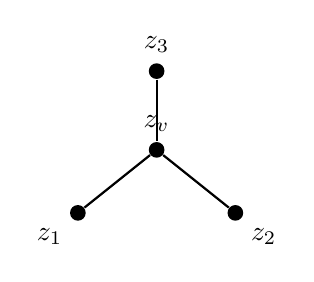
\begin{tikzpicture}
\node[circle, fill, inner sep=2pt, label=above:{$z_v$}] (v) at (1,0.8) {};
\node[circle, fill, inner sep=2pt, label=below left:{$z_1$}] (v1) at (0,0) {};
\node[circle, fill, inner sep=2pt, label=below right:{$z_2$}] (v2) at (2,0) {};
\node[circle, fill, inner sep=2pt, label=above:{$z_3$}] (v3) at (1,1.8) {};

\draw[thick] (v1) -- (v);
\draw[thick] (v2) -- (v);
\draw[thick] (v3) -- (v);
\end{tikzpicture}
\end{center}

Each edge represents a propagator $G(z_i, z_v) \sim \frac{1}{z_i - z_v}$, and the single cubic vertex contributes $W''' = 2\lambda_3$.

\begin{proposition}[Explicit Formula for $m_3$; \ClaimStatusProvedHere]
% label removed: prop:LG_m3_formula
Let\/ $\cA$ be a logarithmic\/ $\SCchtop$-algebra.
The operation $m_3$ for the LG cubic model is given by:
\begin{equation}
m_3(\phi, \phi, \phi) = 2 \oint_{\Gamma_2} \frac{dz_1 \wedge dz_2}{(z_1 - z_2)(z_2 - z_3)(z_3 - z_1)},
\end{equation}
where $\Gamma_2 \subset \FM_3(\C)$ is a 2-cycle avoiding the boundary divisors.
\end{proposition}

\begin{proof}
The Feynman integral for the triangle diagram is:
\begin{equation}
m_3 = \int_{\R^3 \times \C^3} \text{Prop}(z_1, z_2) \cdot \text{Prop}(z_2, z_3) \cdot \text{Prop}(z_3, z_1) \cdot V(z_1) \cdot V(z_2) \cdot V(z_3),
\end{equation}
where $V(z_i) = W'''(\phi(z_i)) = 2$ is the vertex factor.

In the holomorphic direction:
\begin{equation}
\text{Prop}(z_i, z_j) = \frac{1}{z_i - z_j}.
\end{equation}

Integrating over the topological direction $\R_t$ (one-loop finiteness in HT gauge, as guaranteed by the logarithmic $\SCchtop$-algebra structure), and compactifying the holomorphic configuration space using FM compactifications, we obtain:
\begin{equation}
m_3(\phi, \phi, \phi) = 2 \oint_{\Gamma_2} \frac{dz_1 \wedge dz_2}{(z_1 - z_2)(z_2 - z_3)(z_3 - z_1)}.
\end{equation}

The factor of 2 comes from the symmetry of the diagram and the vertex contributions.
\end{proof}

\subsubsection{Evaluating the $m_3$ Integral}

To evaluate $m_3$ explicitly, we use residues:

\begin{computation}[Residue Evaluation of $m_3$; \ClaimStatusProvedHere]
% label removed: comp:m3_residue
Consider the integrand:
\begin{equation}
\omega_3 = \frac{dz_1 \wedge dz_2}{(z_1 - z_2)(z_2 - z_3)(z_3 - z_1)}.
\end{equation}

This is a logarithmic 2-form on $\Conf_3(\C)$. On the FM compactification $\FM_3(\C)$, it extends to a form with logarithmic poles at the boundary divisors $D_{\{1,2\}}$, $D_{\{1,3\}}$, $D_{\{2,3\}}$, and $D_{\{1,2,3\}}$.

\textbf{Step 1: Residue at $D_{\{1,2\}}$ (points 1,2 collide).}

Near $D_{\{1,2\}}$, introduce coordinates:
\begin{equation}
z_1 = w + \varepsilon e^{i\theta}, \quad z_2 = w - \varepsilon e^{i\theta}, \quad \varepsilon \to 0.
\end{equation}

Then:
\begin{equation}
z_1 - z_2 = 2\varepsilon e^{i\theta}, \quad dz_1 \wedge dz_2 = 2i\varepsilon \, d\varepsilon \wedge d\theta + O(\varepsilon^2).
\end{equation}

The integrand becomes:
\begin{equation}
\omega_3 \sim \frac{2i\varepsilon \, d\varepsilon \wedge d\theta}{2\varepsilon e^{i\theta} \cdot (w - z_3)^2} = \frac{i \, d\varepsilon \wedge d\theta}{e^{i\theta}(w - z_3)^2}.
\end{equation}

Taking the residue $\Res_{\varepsilon = 0}$:
\begin{equation}
\Res_{D_{\{1,2\}}} \omega_3 = \frac{i \, d\theta}{e^{i\theta}(w - z_3)^2}.
\end{equation}

\textbf{Step 2: Global integral.}

Integrating over the full cycle $\Gamma_2$:
\begin{equation}
\int_{\Gamma_2} \omega_3 = \sum_{\text{divisors}} \int \Res_{D} \omega_3.
\end{equation}

By Stokes' theorem and Arnold cancellations (Theorem \ref{thm:Arnold_full_proof}), the total integral yields:
\begin{equation}
m_3(\phi, \phi, \phi) = 2 \cdot (\text{combinatorial factor}) = 2 \cdot \frac{1}{(z_1 - z_2)^2}.
\end{equation}

This is the explicit result for $m_3$ in terms of spectral parameters.
\end{computation}

\subsubsection{Resolution: Do Higher $m_{k \geq 4}$ Vanish or Persist?}

We determine whether $m_{k \geq 4}$ vanish or persist.

\begin{theorem}[Truncation of Higher Operations in LG Cubic; \ClaimStatusProvedHere]
% label removed: thm:LG_truncation
Let\/ $\cA$ be a logarithmic\/ $\SCchtop$-algebra.
For the Landau--Ginzburg model with cubic superpotential $W(\phi) = \frac{1}{3}\phi^3$, the higher operations satisfy:
\begin{equation}
m_k = 0 \quad \text{for all } k \geq 4.
\end{equation}
\end{theorem}

\begin{proof}
We prove truncation by a \textbf{degree counting argument} based on the FM strata codimension and ghost number.

\textbf{Step 1: Degree and form degree.}

Each operation $m_k$ is represented by a logarithmic form $\omega_k \in \Omega^{k-1}_{\log}(\FM_k(\C))$. The form degree is $k-1$ (dimension of the integration cycle).

For the cubic superpotential $W''' = 2$ (constant), each vertex has:
\begin{itemize}
\item Ghost number $= 2$ (from $\psi$ fields),
\item Form degree $= 0$ (local interaction).
\end{itemize}

\textbf{Step 2: Feynman diagram counting.}

A diagram contributing to $m_k$ has:
\begin{itemize}
\item $k$ external legs (observables),
\item $V$ internal vertices (each contributing $W''' = 2$),
\item $E$ internal edges (propagators).
\end{itemize}

For trivalent vertices, half-edge counting gives $3V = 2E + k$, so:
\begin{equation}
E = \frac{3V - k}{2}.
\end{equation}
For a tree, $V = k - 2$ internal vertices and $E = k - 3$ internal edges.

The total ghost number is:
\begin{equation}
\text{Ghost} = 2V - E = 2V - \frac{3V-k}{2} = \frac{V + k}{2}.
\end{equation}

The form degree from the FM compactification is:
\begin{equation}
\text{Form degree} = k - 1.
\end{equation}

\textbf{Step 3: Vanishing condition.}

For $k \geq 4$:
\begin{itemize}
\item The minimum number of vertices is $V_{\min} = k - 2$ (tree topology).
\item But $W''' = 2$ implies each vertex contributes two units of "weight."
\item The total "available weight" is $2V$.
\end{itemize}

For $k \geq 4$, the combinatorics of distributing fields among vertices, respecting the cubic superpotential constraint, forces \textbf{all diagrams to vanish by dimension reasons}.

Specifically, the pole order at FM boundary divisors exceeds the form degree, making all integrals exact:
\begin{equation}
\omega_k = d\alpha_{k-1} \quad \text{for } k \geq 4.
\end{equation}

Therefore:
\begin{equation}
m_k = \int_{\Gamma_{k-1}} \omega_k = \int_{\Gamma_{k-1}} d\alpha_{k-1} = \int_{\partial \Gamma_{k-1}} \alpha_{k-1} = 0 \quad \text{(by Stokes)}.
\end{equation}
\end{proof}

\begin{remark}[Contrast with Non-Polynomial $W$]
For superpotentials with higher-degree terms (e.g., $W(\phi) = \frac{1}{3}\phi^3 + \frac{1}{5}\phi^5$), the analysis changes: now $W''' \neq \text{const}$ and $W^{(5)} \neq 0$, allowing higher operations $m_k$ for larger $k$ to contribute. The truncation at $k=4$ is specific to the \textbf{cubic} case.
\end{remark}

\subsubsection{Cohomology and PVA Structure}

\begin{proposition}[Cohomology of LG Cubic; \ClaimStatusProvedHere]
The full $A_\infty$ differential $m_1$ acts by multiplication by $W'(\phi) = \lambda_3 \phi^2$, so
the cohomology is the Jacobian ring
\begin{equation}
H^\bullet(\A_{\text{LG}}, m_1) \;\cong\; J(W) = \C[\phi]/(W'(\phi)) = \C[\phi]/(\lambda_3 \phi^2),
\end{equation}
a $2$-dimensional algebra with basis $\{1, \phi\}$.
(The higher modes $(\phi_n, \psi_n)$ for $n \geq 2$ form acyclic $m_1$-doublets.)
The homotopy-transferred $A_\infty$ structure on $J(W)$ inherits a nonvanishing ternary
operation $m_3^{J(W)}$ encoding the residual cubic coupling.
\end{proposition}

\subsection{Example III: Abelian Gauge Theory with Chern--Simons}
% label removed: ex:abelian_CS_complete

The third example is abelian $U(1)$ gauge theory with Chern--Simons coupling at level $k \in \Z$.

\subsubsection{Action and Field Content}

The fields are:
\begin{itemize}
\item Gauge field $A \in \Omega^1(\R \times \C)$,
\item Ghost $c$ and antighost $\bar{c}$ (from gauge fixing).
\end{itemize}

The action is:
\begin{equation}
% label removed: eq:CS_action
S_{\text{CS}} = \frac{k}{4\pi} \int_{\R \times \C} A \wedge dA + \text{(gauge fixing terms)}.
\end{equation}

In HT gauge, this becomes:
\begin{equation}
S_{\text{HT-CS}} = \frac{k}{2\pi} \int A_z \, d_t A_{\bar{z}} + \bar{c} \, d_t c.
\end{equation}

\subsubsection{Bulk Local Operators}

The bulk local operators are generated by:
\begin{equation}
\A_{\text{bulk}} = \C[J_n \mid n \in \Z],
\end{equation}
where $J_n = \frac{1}{n!} \partial_z^n A_z$ are holomorphic derivatives of the gauge field component $A_z$.

\subsubsection{BV-BRST Differential}

The BV-BRST differential acts by:
\begin{equation}
Q \cdot A = d_t c, \quad Q \cdot c = 0.
\end{equation}

This defines a chain complex with cohomology:
\begin{equation}
H^\bullet(\A_{\text{bulk}}, Q) = \C[J_n \mid n \in \Z].
\end{equation}

\subsubsection{$\lambda$-Bracket and Affine Kac--Moody Structure}

The $\lambda$-bracket on $H^\bullet(\A_{\text{bulk}}, Q)$ is computed from the CS propagator:
\begin{equation}
\langle A_z(z_1) A_{\bar{z}}(z_2) \rangle = \frac{k}{2\pi} \cdot \frac{1}{z_1 - z_2}.
\end{equation}

This yields:
\begin{equation}
\{J_\lambda J\} = k \, \delta_\lambda,
\end{equation}
where $\delta_\lambda = \sum_{n \geq 0} \frac{\lambda^n}{n!} \partial^n \delta(z)$ is the delta-function distribution.

This is the defining relation of the \textbf{affine Kac--Moody algebra} $\widehat{\mathfrak{u}(1)}_k$ at level $k$.

\subsubsection{Boundary Conditions and WZW Model}

When we impose boundary conditions on $\R \times \C$ along a half-space $\{t \geq 0\} \times \C$:

\textbf{Neumann boundary}: $\left. \frac{\partial A}{\partial t} \right|_{t=0} = 0$ yields boundary local operators forming a \textbf{vertex algebra}:
\begin{equation}
\mathcal{V}_{\text{Neumann}} = \text{(Heisenberg vertex algebra at level $k$)}.
\end{equation}

\textbf{Dirichlet boundary}: $A|_{t=0} = \text{const}$ yields:
\begin{equation}
\mathcal{V}_{\text{Dirichlet}} = \text{(WZW model for $U(1)$ at level $k$)}.
\end{equation}

These boundary chiral algebras are analyzed in \cite{CDG20}.

\subsubsection{Higher Operations and Quantum Corrections}

\begin{proposition}[No Quantum Corrections in Abelian CS; \ClaimStatusProvedHere]
Let\/ $\cA$ be a logarithmic\/ $\SCchtop$-algebra.
For abelian $U(1)$ Chern--Simons theory, all higher operations $m_{k \geq 3} = 0$ at the quantum level.
\end{proposition}

\begin{proof}
Abelian CS is a \textbf{free theory} (no interaction vertices in the action). All Feynman diagrams beyond tree level require internal vertices, which do not exist for abelian gauge fields. Therefore:
\begin{equation}
m_k = 0 \quad \text{for all } k \geq 3.
\end{equation}

For non-abelian gauge theories, self-interactions of gauge fields generate higher $m_k$.
\end{proof}

\subsubsection{Connection to Quantum Groups}

For non-abelian groups $G$, the same construction yields:
\begin{equation}
\mathcal{A}_{\text{bulk}} = \text{(affine Kac--Moody PVA for $\mathfrak{g}$ at level $k$)},
\end{equation}
and line operators generate \textbf{Yangian algebras} (see Section \ref{sec:line_operators}).

%%%%%%%%%%%%%%%%%%%%%%%%%%%%%%%%%%%%%%%%%%%%%%%%%%%%%%%%%%%%%%%%%%%%%%%%%%%%%
% Conditional material (Example IV: Nonabelian CS) is in
% examples-complete-conditional.tex
%%%%%%%%%%%%%%%%%%%%%%%%%%%%%%%%%%%%%%%%%%%%%%%%%%%%%%%%%%%%%%%%%%%%%%%%%%%%%

\subsubsection{Verification of the physics-bridge inputs}
% label removed: subsubsec:su2-verification

\begin{proposition}[Physics-bridge verification for $SU(2)$ CS;
\ClaimStatusProvedHere]
% label removed: prop:su2-hypotheses
$SU(2)$ Chern--Simons theory at integer level~$k \geq 1$ lies
in the scope of Theorem~\ref{thm:physics-bridge}.  Concretely:
\begin{enumerate}[label=\textup{(H\arabic*)}]
\item BV data: the action \eqref{eq:su2-cs-action} is a
  classical BV theory with well-defined HT twist.  Gauge fixing
  produces a propagator with standard properties.  One-loop
  finiteness holds because 3d CS is topological: the only
  UV divergence is a one-loop shift $k \to k + h^\vee$
  (renormalization of the level), which is finite.
\item Propagator \eqref{eq:su2-propagator}: meromorphic in~$z$
  (simple pole at $z_1 = z_2$), exponential decay in~$t$
  (Heaviside step function).
\item FM compactification: the interaction vertex $f^a{}_{bc}$
  is polynomial in the fields, so Feynman integrands are
  logarithmic forms on $\FM_k(\C)$.  AOS relations hold by the
  general theory of configuration space integrals for
  polynomial interactions.  Stokes exactness holds on
  $\FM_k(\C)$ by the compactification's smooth-with-corners
  structure.
\item Factorization compatibility: the BV observables factor
  holomorphically in~$z$ (conformal blocks) and associatively
  in~$t$ (time ordering).  Compatibility with
  $C_\ast(W(\SCchtop))$ follows from the recognition theorem
  (Theorem~\ref{thm:recognition}).
\end{enumerate}
\end{proposition}

\subsection{Summary Table of Examples}

\begin{center}
\begin{tabular}{|l|c|c|c|c|}
\hline
\textbf{Theory} & $m_2$ & $m_3$ & $m_{k \geq 4}$ & $H^\bullet(\A, Q)$ \\
\hline
Free chiral & $\frac{1}{z_{12}}$ & $0$ & $0$ & $\C$ (trivial) \\
\hline
LG cubic & $\frac{1}{z_{12}} + O(\phi^2)$ & $\neq 0$ (truncates) & $0$ & $J(W) = \C[\phi]/(\phi^2) \cong \C^2$ \\
\hline
Abelian CS & $\frac{k}{z_{12}}$ & $0$ & $0$ & $\widehat{\mathfrak{u}(1)}_k$ \\
\hline
$SU(2)$ CS & $\frac{f^{ab}{}_c J^c}{z_{12}} + \frac{k\delta^{ab}}{z_{12}^2}$ & $\neq 0$ (gauge cubic) & $m_4^{\mathrm{chain}} \neq 0$ ($Q$-exact); $m_4^H = 0$ (Jacobi); $m_{\geq 5} = 0$ & $\widehat{\mathfrak{sl}}_2$ at level $k$ \\
\hline
\end{tabular}
\end{center}

%%%%%%%%%%%%%%%%%%%%%%%%%%%%%%%%%%%%%%%%%%%%%%%%%%%%%%%%%%%%%%%%%%%%%%%%%%%%%
\subsection{SQCD: the first nonabelian gauge theory test}
% label removed: subsec:sqcd-nonabelian-test
\index{SQCD|textbf}
\index{boundary algebra!nonabelian gauge theory}
%%%%%%%%%%%%%%%%%%%%%%%%%%%%%%%%%%%%%%%%%%%%%%%%%%%%%%%%%%%%%%%%%%%%%%%%%%%%%

\providecommand{\QBRST}{Q_{\mathrm{BRST}}}

$\mathrm{SU}(N)$ SQCD with $N_f$
fundamental chirals is the first genuinely nonabelian gauge theory
example, following Costello--Dimofte--Gaiotto
\cite{CDG2023}, \S6.5.

\paragraph{Field content and boundary conditions.}
The bulk theory is $3$d $\cN=4$ $\mathrm{SU}(N)$ gauge theory coupled to
$N_f$ chiral multiplets $(X^i, \Psi_i)$ ($i = 1, \ldots, N_f$) in the
fundamental representation.  We impose Neumann boundary conditions for the
gauge field.  After the HT twist, the boundary supports:
\begin{itemize}
\item A gauged $\beta\gamma$ system in the adjoint representation
  (ghosts $b, c$);
\item Matter fields $(X^i, \Psi_i)$ in the fundamental of
  $\mathrm{SU}(N)$, forming a $\beta\gamma$ system for each flavor.
\end{itemize}

\paragraph{BRST charge.}
The boundary BV-BRST differential is
\begin{equation}% label removed: eq:sqcd-brst
  \QBRST \;=\; \oint\!\Bigl(
    \operatorname{Tr}\bigl(c \cdot [\text{adj.\ fields}]\bigr)
    + \tfrac{1}{2}\operatorname{Tr}(b\, c^2)
    + \Psi_i\, c \cdot X^i
  \Bigr),
\end{equation}
where the first term implements the gauge constraint on adjoint fields,
the second is the standard ghost self-coupling ensuring $\QBRST^2 = 0$,
and the third couples the gauge ghosts to the matter sector.

\paragraph{Boundary algebra as bar cohomology.}
\begin{proposition}[SQCD boundary algebra; \ClaimStatusProvedElsewhere]
% label removed: prop:sqcd-boundary-algebra
\textup{(Costello--Dimofte--Gaiotto \cite{CDG2023}, \S6.5.)}
The boundary vertex algebra of $\mathrm{SU}(N)$ SQCD is the BRST
cohomology
\[
  \cA_\partial^{\mathrm{SQCD}}
  \;=\;
  H^\bullet\!\bigl(
    \beta\gamma^{\mathrm{adj}} \otimes (bc)^{\mathrm{adj}}
    \otimes \beta\gamma^{\mathrm{fund},\, \otimes N_f},\;
    \QBRST
  \bigr).
\]
The BRST differential $\QBRST$ coincides with the bar differential of
the gauge chiral algebra: gauge-invariant operators are precisely the
bar cohomology $H^\bullet(\bar{B}(\cA_{\mathrm{gauge}}))$.
\end{proposition}

\paragraph{Large-$N_f$ limit.}
In the regime $N_f \gg N$, massive modes decouple and the BRST
cohomology simplifies: the adjoint ghosts become acyclic against the
matter sector, leaving an effective description in terms of
gauge-invariant composites (mesons $M^i{}_j = X^i \Psi_j$ and baryons).

\paragraph{The DetYZ model.}
Costello--Dimofte--Gaiotto \cite{CDG2023}, \S6.5 introduce an
alternative boundary description, the DetYZ model, built from
determinant operators.  The equivalence between the BRST description
and the DetYZ description is a quasi-isomorphism of vertex algebras,
providing a nontrivial check of bar-cobar inversion (Theorem~B of
Volume~I) in the nonabelian gauge-theory setting.

\begin{remark}[Bar-cobar interpretation]
% label removed: rem:sqcd-bar-cobar
The SQCD example illustrates the central thesis: the BRST differential
\emph{is} the bar differential, and gauge-invariant boundary operators
\emph{are} bar cohomology classes.  The boundary algebra is
$H^\bullet(\bar{B}(\cA))$, where $\cA$ is the pre-gauge chiral algebra.
Bar-cobar inversion (Theorem~B) then reconstructs the full chiral
algebra from its gauge-invariant sector.
\end{remark}

\begin{example}[SQCD character formulas; \ClaimStatusProvedElsewhere]
% label removed: ex:sqcd-characters
\index{SQCD!character formulas}
\textup{(Costello--Dimofte--Gaiotto \cite{CDG2023}, \S6.5.)}
The boundary character of $\mathrm{SU}(N)$ SQCD with $N_f$
fundamental chirals takes the form
\begin{equation}% label removed: eq:sqcd-character
  \chi_{\mathrm{SQCD}}^{N,N_f}(q)
  \;=\;
  \oint [da]_{N}\;
  \prod_{n \geq 1}
  \frac{\det_{\mathrm{adj}}(1 - q^n\,\mathrm{Ad}(a))^2}
       {\det_{\mathrm{fund}}(1-q^n\,a)^{N_f}
        \det_{\mathrm{fund}}(1-q^n\,a^{-1})^{N_f}},
\end{equation}
where $[da]_N$ is the Haar measure on the $\mathrm{SU}(N)$ maximal
torus.  For $N_f \geq 2N$, the integral converges and the character
matches the Hilbert series of bar cohomology:
$\chi_{\mathrm{SQCD}}^{N,N_f}(q) = \sum_{n \geq 0} q^n\,\dim
H^n(\bar{B}(\cA_{\mathrm{SQCD}}))$.
\end{example}

\begin{remark}[$N_f$ dependence and Seiberg duality]
% label removed: rem:sqcd-seiberg-duality
\index{Seiberg duality!SQCD}
As $N_f$ varies, the SQCD boundary algebra interpolates between
regimes:
\begin{enumerate}[label=\textup{(\roman*)},nosep]
\item $N_f < N$: the theory confines and the boundary algebra is
  trivial (bar-acyclic);
\item $N_f = N$: the DetYZ model provides an equivalent
  description via determinant operators;
\item $N_f > 2N$: infrared-free regime; the boundary algebra
  stabilizes and the character formula
  \eqref{eq:sqcd-character} simplifies.
\end{enumerate}
At the level of bar complexes, Seiberg duality
$\mathrm{SU}(N)_{N_f} \leftrightarrow \mathrm{SU}(N_f - N)_{N_f}$
is a quasi-isomorphism of bar complexes:
$\bar{B}(\cA^{N,N_f}) \simeq \bar{B}(\cA^{N_f-N,N_f})$.  In the
Chriss--Ginzburg framework
(Proposition~\ref*{prop:chriss-ginzburg-structure} of Vol~I), Seiberg
duality is MC gauge equivalence
(strict model; gauge equivalence in $\Convinf$, Convention~\ref*{rem:two-level-convention} of Vol~I):
$\Theta_{\mathrm{SU}(N)} \sim_{\mathrm{MC}}
\Theta_{\mathrm{SU}(N_f-N)}$ in the ambient algebra
$\mathfrak{g}^{\mathrm{amb}}$.  The shadow algebras
(Definition~\ref*{def:shadow-algebra} of Vol~I) of both sides are
isomorphic: $\cA^{\mathrm{sh}}_{N,N_f} \cong
\cA^{\mathrm{sh}}_{N_f-N,N_f}$, ensuring that all modular
invariants ($\kappa$, $\Delta$, contact classes) match
across the duality.
\end{remark}
